% This file was created with tikzplotlib v0.10.1.
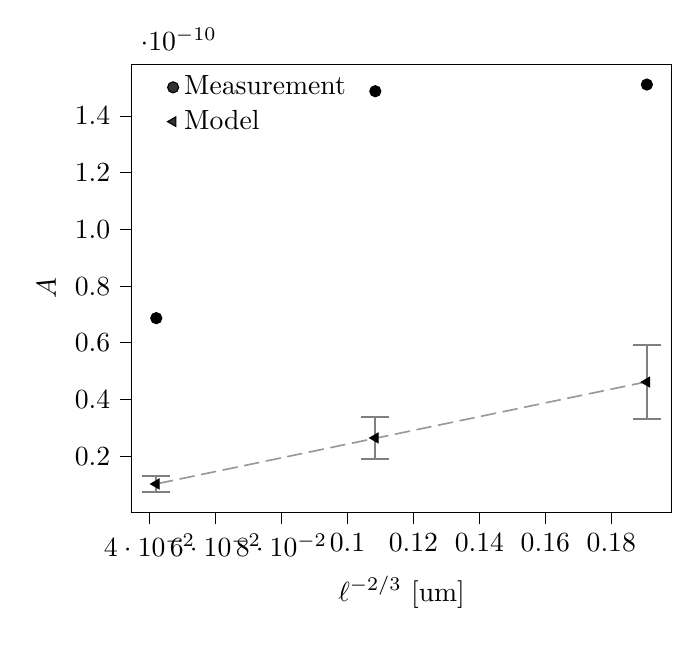
\begin{tikzpicture}

\definecolor{darkgray176}{RGB}{176,176,176}
\definecolor{gray}{RGB}{128,128,128}

\begin{axis}[
legend cell align={left},
legend style={
  fill opacity=0.8,
  draw opacity=1,
  text opacity=1,
  at={(0.05,1)},
  anchor=north west,
  draw=none
},
tick align=outside,
tick pos=left,
x grid style={darkgray176},
xlabel={\(\displaystyle \ell^{-2/3}\) [um]},
xmin=0.0346059638620008, xmax=0.198222837722233,
xtick style={color=black},
y grid style={darkgray176},
ylabel={\(\displaystyle A\)},
ymin=8.85391589976804e-14, ymax=1.58304786968298e-10,
ytick style={color=black},
ytick={0,2e-11,4e-11,6e-11,8e-11,1e-10,1.2e-10,1.4e-10,1.6e-10},
yticklabels={0.0,0.2,0.4,0.6,0.8,1.0,1.2,1.4,1.6}
]
\addplot [draw=black, fill=black, mark=*, only marks]
table{%
x  y
0.190785707092222 1.51113139340602e-10
0.108449606138417 1.48764143206041e-10
0.0420430944920113 6.8679417926444e-11
};
\addlegendentry{Measurement}
\addplot [draw=black, fill=black, mark options={rotate=90}, mark=triangle*, only marks]
table{%
x  y
0.190785707092222 4.61279403531299e-11
0.108449606138417 2.64097960955948e-11
0.0420430944920113 1.01651291626948e-11
};
\addlegendentry{Model}
\path [draw=gray, semithick]
(axis cs:0.190785707092222,3.30364736621996e-11)
--(axis cs:0.190785707092222,5.92194070440601e-11);

\path [draw=gray, semithick]
(axis cs:0.108449606138417,1.89144914439472e-11)
--(axis cs:0.108449606138417,3.39051007472424e-11);

\path [draw=gray, semithick]
(axis cs:0.0420430944920113,7.28018678669314e-12)
--(axis cs:0.0420430944920113,1.30500715386965e-11);

\addplot [semithick, gray, mark=-, mark size=5, mark options={solid}, only marks, forget plot]
table {%
0.190785707092222 3.30364736621996e-11
0.108449606138417 1.89144914439472e-11
0.0420430944920113 7.28018678669314e-12
};
\addplot [semithick, gray, mark=-, mark size=5, mark options={solid}, only marks, forget plot]
table {%
0.190785707092222 5.92194070440601e-11
0.108449606138417 3.39051007472424e-11
0.0420430944920113 1.30500715386965e-11
};
\addplot [semithick, black, opacity=0.4, dash pattern=on 5.55pt off 2.4pt, forget plot]
table {%
0.190785707092222 4.62387588253216e-11
0.180404951786074 4.37228825139288e-11
0.171329908997313 4.15234582424021e-11
0.163316209042784 3.95812606577748e-11
0.15617825056781 3.78513074791021e-11
0.149772318283092 3.6298767917943e-11
0.143985248689135 3.48962157072e-11
0.138726616225864 3.36217353390104e-11
0.133923220198755 3.24575859180444e-11
0.129515114786995 3.13892389956388e-11
0.125452697901677 3.04046730264631e-11
0.121694541564822 2.94938475399203e-11
0.118205751146726 2.86483054854704e-11
0.114956708047904 2.78608685094557e-11
0.111922094572583 2.71254006237738e-11
0.109080129318014 2.6436622895092e-11
0.10641196157244 2.57899666713452e-11
0.103901187194638 2.51814562504683e-11
0.1015334582852 2.46076142804599e-11
0.0992961659781224 2.40653848808608e-11
0.09717818075309 2.35520707049277e-11
0.095169638377507 2.30652810606168e-11
0.0932617623292504 2.26028888730233e-11
0.0914467155991706 2.21629947672857e-11
0.089717476316842 2.17438969252853e-11
0.0880677328182648 2.13440656542904e-11
0.086491794675987 2.09621218242466e-11
0.0849845169095444 2.05968184994456e-11
0.0835412351375521 2.02470252220075e-11
0.0821577098591917 1.99117145079616e-11
0.0808300783896665 1.95899501983395e-11
0.0795548132419223 1.92808773725834e-11
0.0783286859610165 1.89837135834556e-11
0.0771487355896636 1.86977412143595e-11
0.0760122410826703 1.84223007937112e-11
0.0749166971010664 1.81567851284133e-11
0.0738597927090956 1.79006341408651e-11
0.0728393925729927 1.76533303123043e-11
0.0718535203229096 1.74143946504094e-11
0.0709003437910143 1.71833831116102e-11
0.069978161881718 1.69598834189607e-11
0.0690853928657928 1.67435122251053e-11
0.0682205639201212 1.65339125771362e-11
0.0673823017600118 1.63307516462445e-11
0.0665693242322528 1.61337186902156e-11
0.0657804327550435 1.59425232211734e-11
0.06501450550619 1.57568933546743e-11
0.0642704912739312 1.55765743193946e-11
0.06354740389584 1.54013271093453e-11
0.0628443172207326 1.52309272628417e-11
0.0621603605366624 1.50651637544338e-11
0.0614947144150852 1.49038379876994e-11
0.0608466069273321 1.47467628782699e-11
0.0602153101947615 1.45937620177262e-11
0.0596001372384988 1.44446689101029e-11
0.0590004390986181 1.42993262736939e-11
0.0584156021960567 1.41575854016871e-11
0.0578450459135534 1.40193055758813e-11
0.057288220374526 1.38843535283759e-11
0.0567446044011049 1.37526029466803e-11
0.0562137036345598 1.36239340181814e-11
0.0556950488031373 1.34982330103373e-11
0.0551881941238914 1.33753918833455e-11
0.0546927158264794 1.32553079323704e-11
0.0542082107881157 1.31378834567113e-11
0.0537342952699678 1.30230254535559e-11
0.0532706037462377 1.29106453341964e-11
0.0528167878180355 1.2800658660797e-11
0.0523725152049096 1.26929849019808e-11
0.0519374688075854 1.25875472056759e-11
0.0515113458360682 1.24842721878026e-11
0.0510938569978123 1.23830897355184e-11
0.0506847257411486 1.2283932823855e-11
0.0502836875495956 1.21867373446885e-11
0.049890489283077 1.20914419470762e-11
0.0495048885624186 1.19979878880844e-11
0.0491266531938193 1.19063188933026e-11
0.0487555606302759 1.18163810263152e-11
0.0483913974672012 1.17281225664594e-11
0.0480339589697103 1.16414938942581e-11
0.0476830486292608 1.15564473839684e-11
0.0473384777475269 1.14729373027283e-11
0.0470000650455585 1.13909197158334e-11
0.0466676362964397 1.13103523977078e-11
0.0463410239797983 1.12311947481714e-11
0.0460200669566569 1.11534077136366e-11
0.0457046101632282 1.10769537128969e-11
0.04539450432237 1.1001796567195e-11
0.0450896056715146 1.09279014342842e-11
0.0447897757059761 1.0855234746216e-11
0.044494880936623 1.07837641506101e-11
0.0442047926609806 1.07134584551788e-11
0.043919386746895 1.06442875752955e-11
0.0436385434279557 1.05762224844139e-11
0.0433621471099329 1.0509235167156e-11
0.0430900861875367 1.04432985749018e-11
0.0428222528708587 1.03783865837259e-11
0.0425585430208974 1.03144739545354e-11
0.0422988559936155 1.02515362952759e-11
0.0420430944920113 1.01895500250793e-11
};
\end{axis}

\end{tikzpicture}
